% The FYP template is designed according to NTU SCSE FYP guidelines on https://www3.ntu.edu.sg/scse/fyp/UsefulInfo/Report%20Guide.pdf.

\documentclass[pdftex, 12pt, a4paper]{article}
\usepackage{newtxtext, newtxmath}
\usepackage[top=3cm, bottom=3cm, left=3.5cm, right=3cm]{geometry}
\usepackage[hidelinks]{hyperref}
\usepackage[pdftex]{graphicx}
\usepackage{booktabs}
\usepackage{setspace}
\usepackage{titlesec}
\usepackage{tocloft}
\usepackage{parskip}
\usepackage{amsmath}
\usepackage{amsfonts}
\usepackage[sorting=none]{biblatex}

\usepackage[linesnumbered, ruled,vlined]{algorithm2e}
\usepackage{algorithmic}

\usepackage{multirow}
\usepackage[acronym]{glossaries}
\loadglsentries{glossaries}

\addbibresource{bib.bib}
\setstretch{1.5}
\setlength{\cftfigindent}{0pt}
\setlength{\cfttabindent}{0pt}
\renewcommand{\cftdotsep}{1}

% change the following
\title{\uppercase{Graph spectral partitioning
}}

\date{Spring 2023}

\begin{document}
\makeatletter
\begin{titlepage}
\begin{center}

\uppercase{\textbf{\large{Hanoi University Of Science and Technology}}}
\\[5cm]

{{\Large{Technical report}}}
\\[0.5cm]
\uppercase{\textbf{\Large{\@title}}}
\\[2cm]

by \\
\Large{Le Van Cuong}\\
\normalsize{\url{cuong.lv212179M@sis.hust.edu.vn}}\\[1cm]

Supervised by \\
\Large{Dr. Nguyen Kiem Hieu}\\


\vfill
\normalsize{\@date}

\end{center}
\end{titlepage}
\makeatother

\setcounter{page}{1}

\pagebreak

% \tableofcontents

\section{Introduction}
The spectral partitioning algorithm \cite{pothen1990partitioning} was proposed in the context of computing a good ordering for the parallel factorization of sparse and symmetric matrices. 
The purpose is to distribute the work of matrix operations across multiple processors or computing nodes in a parallel computing system. Due to the computational efficiency, spectral partitioning has been used widely for graph partitioning. 
The algorithm is based on the eigenvalues (spectrum) and eigenvectors of the graph's Laplacian matrix to divide the graph into two or more disjoint subsets, or partitions. Generally, the Laplacian matrix of the graph is first constructed from the adjacency matrix and the degree matrix. The eigenvalues and eigenvectors of the Laplacian matrix are then computed, and based on these, the graph is divided into two initial partitions. Based on the edge separator (i.e., the set of all edges that connect the partitions), the vertex separator is calculated by a maximum matching.

The goal of this project is to understand how the spectral partitioning algorithm works and to re-implement it. According to the descriptions in the paper, the algorithm is implemented in C++ and the obtained results are identical to those reported by the authors. The source code is available at \url{https://github.com/cuonglvsoict/Graph-spectral-partitioning}, while the matrices used in the experiments can be found at \url{https://math.nist.gov/MatrixMarket/}.

\section{Preliminaries}
This section briefly introduces the graph partitioning problem and fundamentals of spectral graph theory.

\textbf{Graph partitioning problem}: Given an undirected graph $G = (V, E)$ on $|V| = n$ vertices indexed by \{1, 2, \ldots, n\}. The goal is to find a vertex separator $S$ that disconnects $G\symbol{92}S$ into two parts (partitions) $A$ and $B$ such that $|S|$ and the cardinality difference between $A$ and $B$ are minimized.

Let $A$ be the $n \times n$ adjacency matrix $G$. Then, $A$ is given by
\[
    a_{uv} = \begin{cases}
    1, & \text{if } (u, v) \in E\\
    0, & \text{otherwise}.
    \end{cases}
\]
By convention, we let $a_{uu} = 0$ for all $u \in V$.
Let $D$ be the $n\times n$ degree matrix of $G$. Then, $D$ is a diagonal matrix where $d_{uu}$ is the degree of the vertex $u \in V$. Given $A$ and $D$, the Laplacian matrix of the graph $G$ is defined by $L = D - A$. Let $\lambda_1, \lambda_2, \ldots, \lambda_n$ be the eigenvalues of $L$. The eigenvalues have some important characteristics as follows
\begin{itemize}
    \item $L$ has real eigenvalues $\lambda_1 = 0 \leq \lambda_2 \leq \ldots \leq \lambda_n$.
    \item The number of zero eigenvalues of $L$ is equal to the number of connected components of $G$. Thus, if $G$ is connected graph then we have $\lambda_2 > 0$.
\end{itemize}
The second eigenvalue $\lambda_2$ is called algebraic connectivity, which related to the vertex and edge connectives of the graph $G$. Let $\mathbf{x} \in \mathbb{R}^n$ be the eigenvector corresponding to the eigenvalue $\lambda_2$. The next section shows how $\mathbf{x}$ is used to partition the graph $G$.

\section{Spectral partitioning algorithm}
\label{sec:algo}
Recall, our goal is to partition the vertices of $G$ into two subsets $A$ and $B$ with nearly equal sizes, and the vertex separator $S$ as small as possible. The spectral partitioning algorithm is as follows.
\begin{itemize}
    \item[\textit{Step 1.}] Construct the Laplacian matrix $L$ of graph $G$. Calculate the eigenvector $\mathbf{x}$ corresponding to the second eigenvalue $\lambda_2$. Calculate the median value $x_m$ of elements of $\mathbf{x}$.
    \item[\textit{Step 2.}] Based on $\mathbf{x}$ and $x_m$, divide $V$ into two initial partitions, let say, $A'$ and $B'$. The subset $A'$ includes all vertices $i \in V$ with the corresponding component in the eigenvector $x_i \leq x_m$. The subset $B'$ consists of all vertices $i\in V$ with $x_i > x_m$. If there are multiple vertices $i$ with $x_i = x_m$, randomly assign them to $A'$ an $B'$ in such a way that $\big||A'| -|B'|\big| \leq 1.$
    \item[\textit{Step 3.}] Extract the edge separator $E'$ including all the edges with one endpoint in $A'$ and the other in $B'$. Let $A_1$ be the set of endpoints belonging to $A'$ and $B_1$ be the set of endpoints belonging to $B'$. Then we have a bipatite $H = (A_1, B_1, E')$.
    \item[\textit{Step 4.}] Calculate the vertex separator $S$ of $G$ by finding the minimum vertex cover of the bipartite $H$. The minimum cover of $H$ can be found through finding a maximum matching of $H$, which can be done in polynomial time since $H$ is a bipartite.
    \item[\textit{Step 5.}] Calculate the graph' partitions as $A = A'\symbol{92}S$ and $B = B'\symbol{92}S$.
\end{itemize}

\section{Numerical results}
This section presents the numerical results to validate the implementation.

\subsection{Results on small test instances}

Two small graphs are constructed for testing during the implementation and visualization. The results obtained from the implemented algorithm are plotted in Figure \ref{fig:result_small}. The figure shows that the algorithm successfully partitions the graphs into subsets such that the size of the separators $S$ are minimized.

\begin{figure*}[t]
\begin{minipage}{0.49\textwidth}
    \centering
    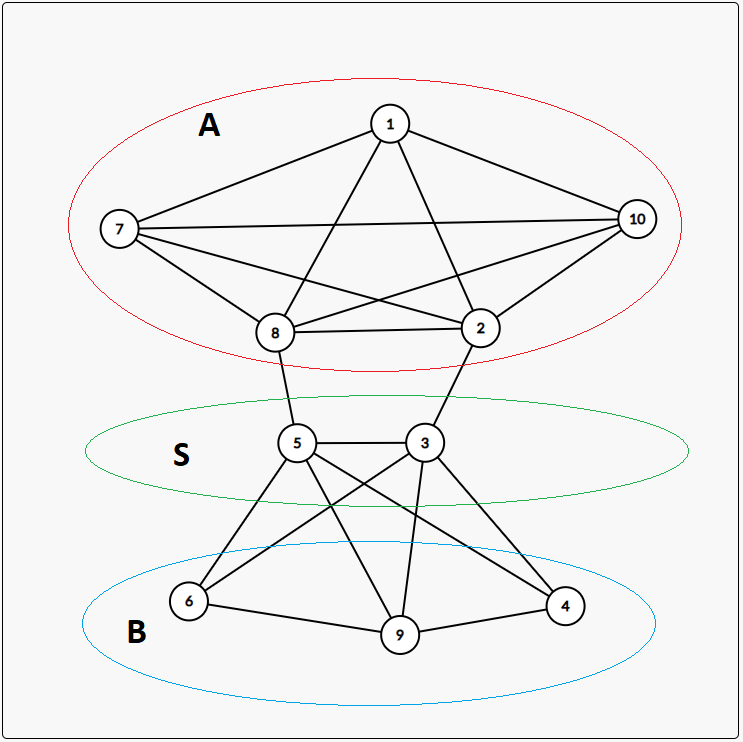
\includegraphics[width=\textwidth]{figures/small_test1.PNG}
\end{minipage}
\hfil
\begin{minipage}{0.49\textwidth}
    \centering
    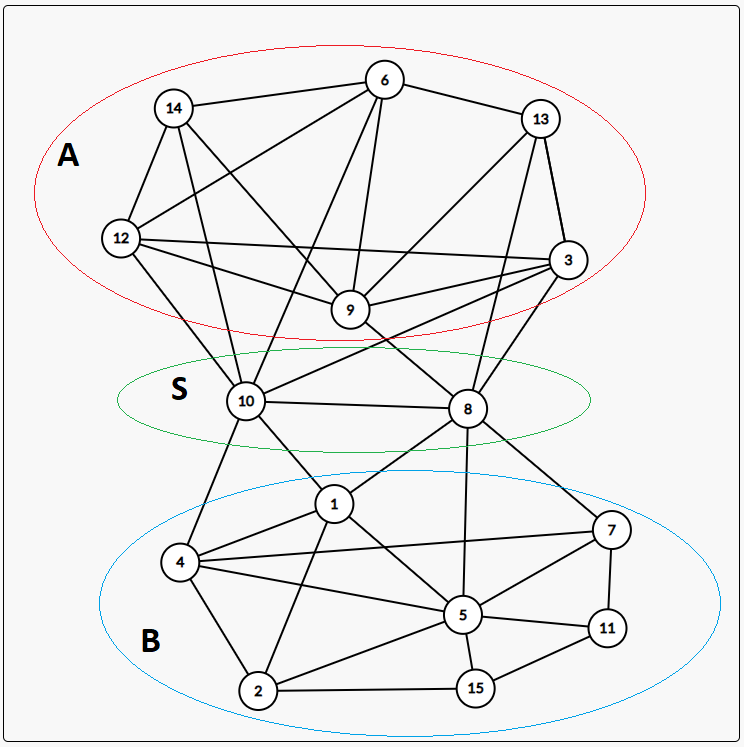
\includegraphics[width=\textwidth]{figures/small_test2.PNG}
\end{minipage}
\caption{Results on small test instances, where $A$ and $B$ are two graph partitions and $S$ is the vertex separator.}
\label{fig:result_small}
\end{figure*}

\subsection{Results on datasets used in the original paper}
This subsection reports the experimental results on several datasets that have been used by the authors in \cite{pothen1990partitioning}. Noting that the stochastic factor of the spectral partitioning algorithm arises in \textit{Step 3} (see, section \ref{sec:algo}), where there may exist multiple vertices $i \in V$ with their corresponding components in the second eigenvector equal to the median value $x_m$, and these vertices are randomly assigned into two initial partitions $A'$ and $B'$. However, this is unlikely to happen in reality due to the nature of the eigendecomposition in \textit{Step 1}. Therefore, the algorithm could be considered as a deterministic algorithm, and if the implementation is correct, the obtained results should be identical to the results reported in \cite{pothen1990partitioning}.

Five test instances are used in this experiments, i.e., five matrix graph downloaded from \url{https://math.nist.gov/MatrixMarket/}. The results are tabulated in Table \ref{tab:main_results}, where the obtained partitions and vertex separators have the same size as in the original paper, i.e., Table 1 in \cite{pothen1990partitioning}. 

\begin{table}[]
\centering
\caption{Results on datasets used in the original paper}
\label{tab:main_results}
\begin{tabular}{@{}lllllllll@{}}
\toprule
\multicolumn{1}{c}{\multirow{2}{*}{Dataset}} &  & \multicolumn{3}{c}{Implemented   by authors} &  & \multicolumn{3}{c}{Re-implemented} \\ \cmidrule(lr){3-5} \cmidrule(l){7-9} 
\multicolumn{1}{c}{}                         &  & $|S|$ \qquad \quad        & $|A|$ \qquad \quad         & $|B|$           &  & $|S|$\qquad \quad       & $|A|$ \qquad \quad       & $|B|$       \\ \midrule
BCSPWR09                                     &  & 20           & 857           & 846           &  & 20        & 857        & 846       \\
BCSPWR10                                     &  & 31           & 2623          & 2646          &  & 31        & 2623       & 2646      \\
BCSSTK13                                     &  & 236          & 862           & 905           &  & 236       & 862        & 905       \\
CAN 1072                                     &  & 33           & 525           & 514           &  & 33        & 525        & 514       \\
JAGMESH                                      &  & 26           & 442           & 468           &  & 26        & 442        & 468       \\ \bottomrule
\end{tabular}
\end{table}


\printbibliography[title={References}]

\end{document}